\section{Frontend}
\label{sec:Insieme.Frontend}

The frontend of the compiler is responsible of parsing an input program written
in a specific input language and to produce an IR program which semantically
equivalent to the input code. Because the IR is generic, many different input
programming languages can be represented by it. However a frontend must be
specific to an input language.

In the current development stage of the Insieme compiler only one frontend
exists for C-like languages based on the LLVM/Clang compiler~\cite{clang}. This
frontend supports C and C++, and above that it can deal with C language
extensions which are for example utilized for OpenCL and OpenMP. Because the
language extensions are always defined on top of a valid C/C++ code, the frontend
parse the input code in 2 major steps. In the first step, the sequential part of
the code is treated and converted into IR data structures. During this process,
information of eventual code extensions is collected and stored internally to
the frontend. In the second step, language extensions encountered in the input
code are applied to the generated IR and the final IR program is produced.  

\subsection{Overview of the Insieme Frontend}
\label{sec:Insieme.Frontend.Overview}

The frontend's job is to convert the AST generated by the LLVM/Clang compiler
into the corresponding IR DAG. Before this conversion can take place, the AST of
an input C/C++ code has to be generated. An overview of the conversion chain
implemented in Insieme is depicted in Figure~\ref{fig:Frontend.Architecture}.
The major difference between how any C compiler works and Insieme starts here.
While a generic C compiler parses, analyzes and compiles each translation unit
of the input program separately (often for performance reasons); Insieme needs
to have the knowledge of the entire input program before the conversion can be
started. For example, in order to be constructed, a \texttt{CallExpr} node of
the IR needs a reference to the corresponding \texttt{LambdaExpr} node which
contains the body of the invoked function.  Therefore the \texttt{CallExpr} node
cannot be created before the invoked function has been converted. Because a
function body in a C program often refers to a function definition in a
different translation unit, all the content of the translation units composing
the input program needs to be collected before the IR conversion process can
start.  This part will be discussed in more details in
Section~\ref{sec:Insieme.Frontend.TranslationUnits}.

\begin{figure}[tb]
	\centering
	%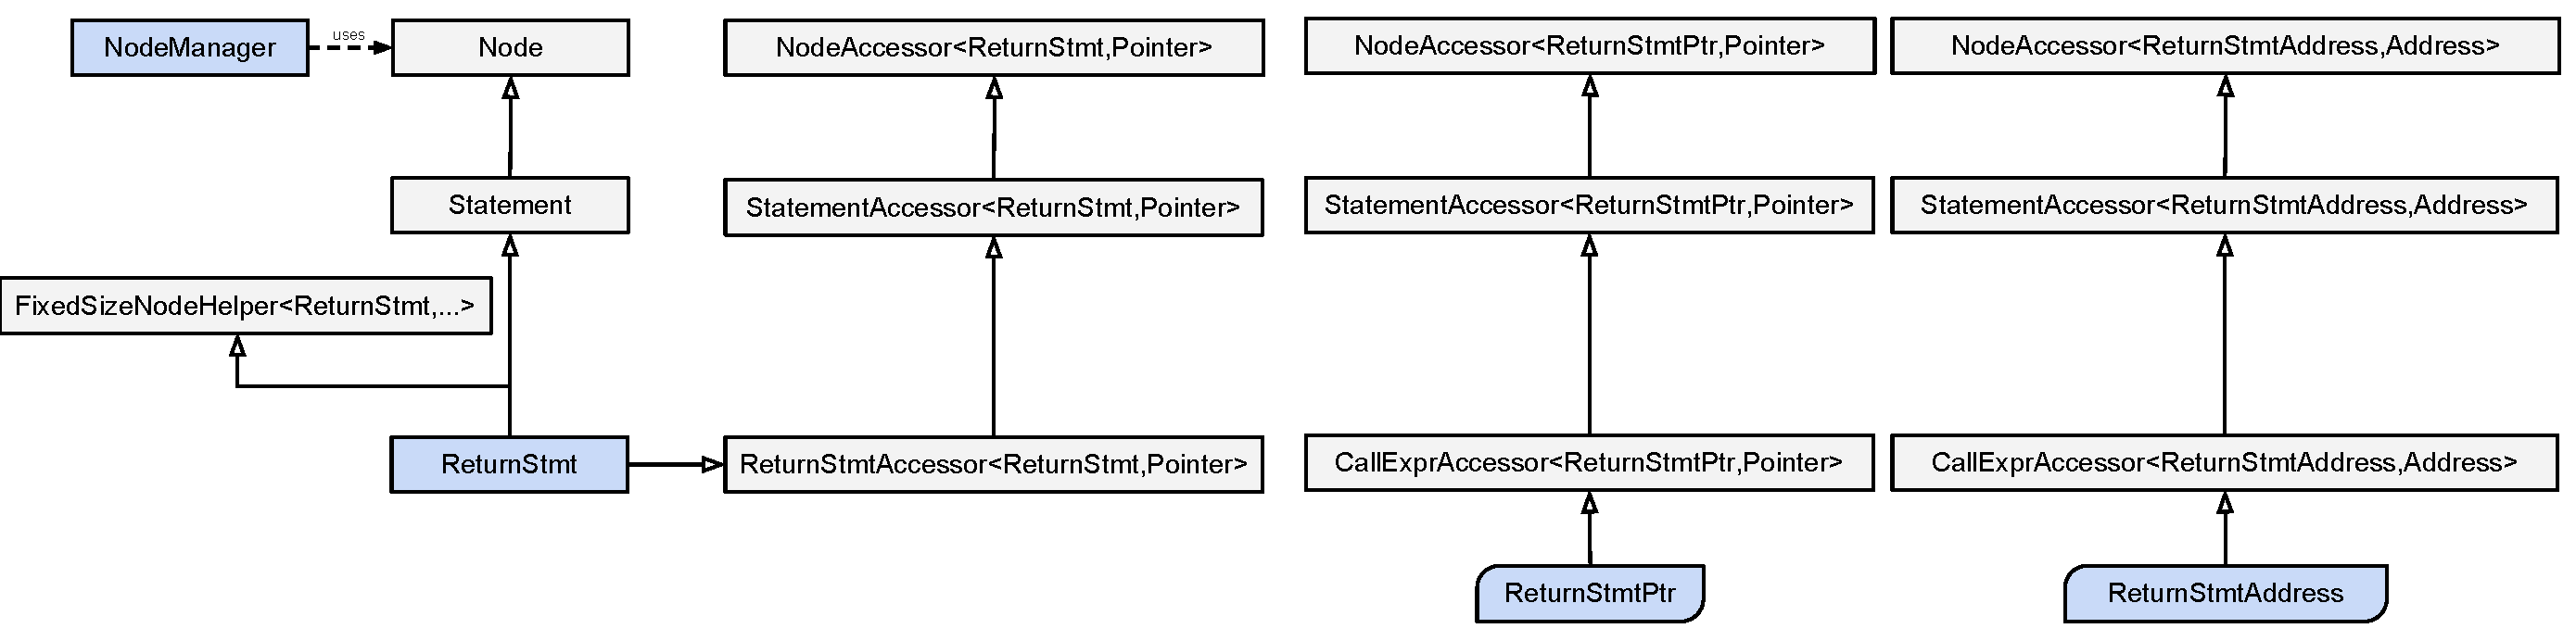
\includegraphics[width=\textwidth]{compiler/core/class_hierarchy_of_return_stmt.pdf}
	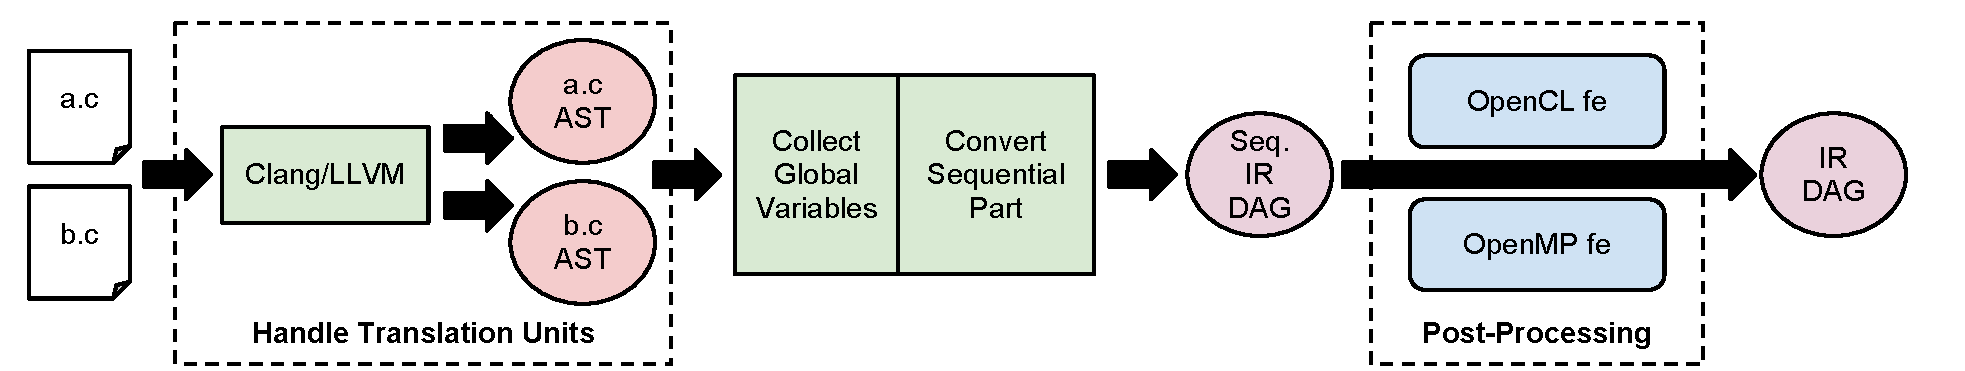
\includegraphics[width=\textwidth]{compiler/frontend/architecture.pdf}
	\caption{Overview of the frontend architecture}
	\label{fig:Frontend.Architecture}
\end{figure}

Once all translation units AST are in memory an analysis step on the entire
program is performed to capture eventual global and static variables in the
input code.  Indeed, because of the structural nature of the INSPIRE language,
variables are not referred by their name but instead by the DAG node
representing that variable. This makes it difficult to handle the semantics of
C/C++ \emph{global} and \emph{static} variables. In order to create a valid, and
semantically equivalent, IR program, the frontend needs to remove every global
variable from the program and accordingly replace them with plain variables
taking care of maintaining the semantics of the code. The details and
implementation issues related to the analysis phases performed for this issue
are discussed in Section~\ref{sec:Insieme.Frontend.Global}. 

Conversion of the Clang AST into an IR DAG is done using the well established
``Visitor'' design pattern~\cite{visitor-pattern}. The main idea is, for each
node of the Clang AST, to provide a transformation function which describe how
the C language entity (e.g. a variable declaration, an expression) should be
represented in the INSPIRE intermediate representation.  Management code makes
sure the generated IR nodes are automatically/correctly composed into a DAG. The
conversion of AST nodes of the C/C++ language is separated (for readability
issues) into 4 modules. 
\begin{description}
\item [{\tt TypeConverter}] takes care of converting C/C++ data types (e.g. int,
array, struct) into the
corresponding IR types;
\item [{\tt StmtConverter}] takes care of converting C statements (e.g. for, if,
switch) into the corresponding IR statements;
\item [{\tt ExprConverter}] converts C expressions into IR expressions;
\item [{\tt CxxConverter}] Converts C++ specific entities (e.g. virtual method
calls) into an IR representation.
\end{description}
These four modules are managed by the {\tt ConversionManager} which is described
in Section~\ref{sec:Insieme.Convert}
While the conversion of most of the C AST nodes is straightforward and heavily
documented in the source code, one of the challenges in the frontend is the way
recursive types and functions are generated. Handling of such problem is treated
in Section~\ref{sec:Insieme.Recursion}.

One of the major features, and efforts, of the Insieme frontend is the handling
of user pragmas. Indeed, as part of the Insieme project, an engine for pragma
matching on top of the Clang compiler was developed. This framework allows for
user pragmas to be defined in EBNF form. The engine takes care of matching those
pragmas and store in a separate data structure, as node annotations, the pragma
information for later consumption~\ref{sec:Insieme.Pragmas}. A use case is the
implementation of the entire OpenMP 3.0 standard on top of our
framework~\ref{sec:Insieme.OpenMP}. 

\subsection{Handling of Translation Units}
\label{sec:Insieme.Frontend.TranslationUnits}
\todo{week24}

\subsection{Handling of Global Variables}
\label{sec:Insieme.Frontend.Global}
\todo{week24}

\subsection{Conversion Manager}
\label{sec:Insieme.Convert}
\todo{week25}

\subsection{Recursive Type and Functions}
\label{sec:Insieme.Recursion}
\todo{week26}

\subsection{Matching of User Pragmas}
\label{sec:Insieme.Pragmas}
\todo{week27}

%\subsection{OpenCL Frontend}
\label{sec:Insieme.OpenCL}

The OpenCL part of the Insieme frontend has two major responsibilities: On one hand it implements the semantics of many OpenCL library calls (in the OpenCL host code) and OpenCL built-in functions and implicit semantics (in the device code) to enable advantageous prgogram analysis. On the other hand, it connects the host and device code of an OpenCL program to form one single instance. Doing so, a lot of analysis and transformations can be done, which would not be possible when looking a both parts individually. One goal of the OpenCL frontend is to make all functinalities of the OpenCL library and built-in functions explicit, so that it an OpenCL program could be translated to a C program with the same semantics. \\

The transformations performed by the OpenCL frotnend are done entirely on INSPIRE level. This means, that the generic C/C++ frontend generates an IR DAG from the source code on which the OpenCL frontend performs some transformations, as shown in Figure~\ref{fig:Frontend.Architecture}. Qualifiers (e.g. \texttt{\_\_kernel}, \texttt{\_\_local}, \texttt{\_\_global}, etc.) which are not part of standard C are translated to \texttt{annotations::ocl::BaseAnnotation} with inside another annotation from the \texttt{annotations::ocl} namespace, depending on the qualifier (see Section~\ref{sec:Compiler.Core.Annotations} to read how and why annotations contain other annotations). The generic frontend is also responsible to translate OpenCL vector types to INSPIRE vectors with the appropriate type as well as translating vector accesses to subscript operations and operations on vectors (e.g. addition) to calls to the function \texttt{vector.pointwise}. This is done directly when translating the Clang AST to the INSPIRE DAG. \\

Since the OpenCL host code is just a standard C/C++ code which includes some specific headers whereas the device or kernel code uses an extension to a subset of C, the OpenCL frontend for both parts are implemented in two completely independend components which will be described in the following paragraphs. \\


\subsubsection{OpenCL Device Frontend}
\label{sec:Insieme.DeviceCL}

To be able to compile an OpenCL kernel function with Insieme, its file must include \texttt{ocl\_device.h}. This header file declares (but not implements) most of the OpenCL built-in functions, in both scalar and vector version. Since Clang version 3.0 the frontend shows some warnings about redeclaring some functions, since they are now built-in in Clang to. However Clang includes only very few functions, and of them it declares only one interface. Therefore this header file is still needed. When this header file is included in a kernel file, it cannot be compiled with an OpenCL compiler any more, since redefining all built-in funcitons leads to an error. Therefore it is a good practice to wrap the include inside \texttt{\#ifdef INSIEME} and to pass this definition to the call of the insieme compiler. 

Since the OpenCL kernels do not have a main function, the compiler is not able to find the entry points automatically. Therefore one must mark all kernel functions that should be compiled with Insieme using \texttt{\#pragma insieme mark}. The generic frontend will then generate a program with a separate entry point for each kernel functions and add an annotation which will be described in the next paragraph.

The transfromations necessary for the OpenCL device code are done in \texttt{ocl\_compiler.cpp}. The transformations are invoked by creating an object of type \texttt{insieme::ocl::Compiler} and invoking it's function \texttt{lookForOclAnnotations}. This functions walks through the program passed to its classe's constructor and searches for Nodes of type \texttt{NT\_MarkerExpr} which hold an \texttt{annotations::ocl::BaseAnnotation} with inside a \texttt{annotations::ocl::KernelFctAnnotationPtr}. This annotation is added by the C frontend to all functions which feature the OpenCL \texttt{\_\_kernel} qualifier. \\

When such a node is found the OpenCL host code transformations start on the child of the Marker Node. During these transformations the Marker Node itself will be removed while it's child will be replaced with a transformed version of it. The previously found \texttt{annotations::ocl::BaseAnnotation} will be attached to this newly generated node without any changes. \\

The most important task of the device frontend is to make the implicit parallelism of OpenCL explicit. When calling an OpenCL kernel, several instances of it will be started in a two level hirarchy of threads. The instances of the first level is called groups. Those gropus cosist of several work items (which are similar to threads). Both levels can have up to three dimensions. For a detailed description see~\cite{oclRef}. In order to capture this semantics in IR, two nested \texttt{parallel/job} constructs~\ref{parallel}[add ref to parallel constructs here] are wrapped around the kernel function's body, one covering the parallel groups, the other the parallel work items. Those \texttt{job} have a fixed range which is determined by the arguments \texttt{global\_work\_size} and \texttt{local\_work\_size} of the function \texttt{clEnqueueNDRangeKernel}. In OpenCL these values are passed to the kernel function impicitly, therefore in OpenCL we need to add two more arguments to the kernel to pass them explicitly. The number of theads of the outher parallel is equal to \texttt{global\_work\_size / local\_work\_size}. Therefore at the beginning of the kernel function, a statement performing exactly this calculation is added in order to use this as argument to the outher \texttt{job}. \\

The \texttt{parallel/job} constructs in INSPIRE are only one dimensional. Therefore the three dimensional thread grid of OpenCL simply flattend to generate two one dimensional spaces. In order to maintain the semantics of the input program, the three dimensional group/local or global id has to be restored at any place where an instance of \texttt{get\_[group|local|global]\_id} is called. In oder to do so, these functions are replaced with new functions, implemented in Inspire. Those new functions take not only the dimenson as argument (as their OpenCL counterparts do), but also the local/global size (passed as arguments to the kernel function as described in the prevous paragraph) and/or number of groups (calculated at the first line of the kernel, as described in the prevous paragraph), depending on the actual function. From these parameters the actual, 3D index is calculated using division and modulo calculations. Similarily, calls to \texttt{get\_[local|global]\_size} and \texttt{get\_num\_groups} are replaced with functions implemented in INSPIRE to give the same return value as the original ones.

Since adding \texttt{parallel/job} constructs introduces new scopes in INSPIRE, new variables have to be introduced in order to bring the values of the parameters of the kernel function to its body. The OpenCL Device Frontend does this 'bottom up' which means, that the ids of the variables inside the kernel body remain unchanged, while new variables are generated to be used in the parallel calls and as arguments. Furthermore, arguments which use the \texttt{\_\_local} or \texttt{\_\_constatnt} qualifier are added to the shared variable list of the jobs. Variables with a \texttt{\_\_global} qualifier are not added, since they are always pointer, and the pointer itself is private, only the data it is pointing to is shared among all treads. The declaration of local variables which use the \texttt{\_\_local} qualifier inside the kernel's body are moved between the two \texttt{parallel/job} constructs and the corresponding variables are added to the arguments of the inner \texttt{parallel} as well as to the shared variable list of the inner \texttt{job} to match the OpenCL semantics. 

When inside a kernel another function is called, the interface of this function may be changed. As mentioned before, in the INSPIRE represenation some functions need the local, global or group variable as argument which is not there in the OpenCL input code. Therefore, if anything inside a subfunction needs one of those variables, they will be added to the its interface and call.

In OpenCL all math functons (e.g. sin, cos etc.) can be marked as \texttt{native\_}. This keword means that, if awailable, a faster and less accurate version of the function (usually implemented in hardware) shall be used. To cover this semantic, the OpenCL Host Frontend removes the native from the function call and embeds it in a call to the function \texttt{accuracy.fast}, to keep the information that accuracy should be traded for speed if possible. This is also done for math functions marked as \texttt{half\_}. In OpenCL they use only two byte floating point numbers. But since Insieme does not support those and translates them to four byte floats, at least the fact that this function does not need high accuracy is preserved. The same is done for \texttt{mul24}. Since INSPIRE does not support \texttt{fma}, this function is expanded into a multiplication and an addition.

\texttt{mem\_fence} in OpenCL are directly translated into calls to \texttt{barrier} in INSPIRE. Mem fences on the local scope are mapped to barriers on the inner parallel while mem fences on global scope correspond to barriers on the outher (and therefore also inner) parallel region.

In OpenCL it is legal to assign a pointer of type \texttt{int} to another pointer of vector-type \texttt{int4} by using a simple cast. However this does not correspond with the semantics of a \texttt{CAST} in INSPIRE. Therefore, in such operations are replaced with a call to the function \texttt{ref.reinterpret}. This is already done in the generic frontend during the translation from Clang AST to the INSPIRE DAG. When one of the function starting with \texttt{convert\_} is used to transform scalar arrays to vectors, this function is not affected by the generic frontend but passed to the OpenCL Device Frontend. There it is replaced with a function which iterates over the array and constructs the desired vector element wise. Note: the function \texttt{ref.reinterpret} can not be applied here in general, since the soure may be not a reference.




\subsubsection{OpenCL Host Frontend}
\label{sec:Insieme.HostCL}



\subsection{OpenMP Frontend}
\label{sec:Insieme.OpenMP}



